% Motivation

\chapter{Einleitung}\label{Einleitung}
Hier gehört die Einleitung/Motivation hin. Auf Kapitel \ref{Einleitung} kann so verwiesen werden.

\section{Nötige Programme}
Für die Arbeit mit Latex benötig man eine Tex-Distribution, verbreitet sind hier Miktex und TExlive, empfohlen wird Texlive(\url{https://www.tug.org/texlive/}) in der aktuellsten Version(Upgraden!).

Außerdem benötig man einen Editor, verbreitet sind hier Texniccenter, Texmaker, TexmakerX und Texstudio. Empfohlen wird Texstudio(\url{http://www.texstudio.org/}).

Für die Literaturverwaltung (Erstellen der Bibfiles )kann ein einfacher Texteditor(Notepad++) Texstudio oder (für poweruser) jabref  verwendet werden.


\section{Einige tex Kommandos}\label{sec:texkommandos}
\markboth{Einige tex Kommands}{Einige tex Kommands} %für die kopfzeile

Auf eine Überschrift \ref{sec:texkommandos} kann so verwiesen werden. Unter jedem Kapitel und jeder Überschrift sollte zumindest ein Satz Text stehen.

\subsection{Unterüberschrift}
Je kleiner, desto mehr "`sub"'s kommen davor.

\subsection{Bilder und Quellen}

Auf ein Bild kann mit Abb. \ref{fig:textreferenz} verwiesen werden. Dies sollte immer passieren, bevor es im erscheint. Einige Beispielplots finden sich außerdem im Anhang.

%empfänger
\begin{figure}[h] %h(ere), t(op), b(ottom) stehen für den ort an dem das bild wenn möglich erscheint. ! und großschreibung sind strikter. bei htb wird zuerst das h beachtet, dann das t usw
\centering
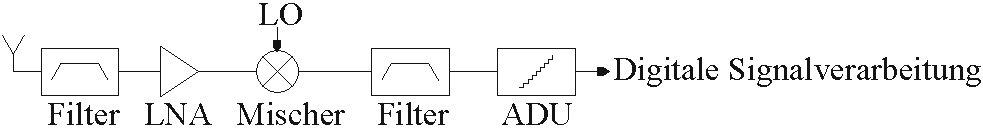
\includegraphics[width=14cm]{XX_DEMO_empfaenger} %Größe, Ort, am besten als vektorgraphik (pdf), Photos als jpg
\caption{Beschreibung (Quellen dahinter) \cite{BibDEMO1}\cite{BibDEMO2}}
\label{fig:textreferenz}
\end{figure}

Eine Quelle wird direkt hinter dem Satz vor dem Punkt angegeben mit \cite{BibDEMO1}, oder aber hinter einem kompletten Absatz. Auch Formeln (im Text) und Bilder (in der caption) müssen eine Quellenangabe enthalten.

Schöne Schaltpläne lassen sich auch direkt in Latex mi tikz/circuitikz malen, siehe \ref{tikz}.

\begin{figure}
	\centering
	\tikzsetnextfilename{XX_DEMO_tikz} %Dateiname, unter der die datei im ordner tikz-ext-out angelegt wird
	\tikzset{external/remake next} %uncomment to force remake figure
	\begin{tikzpicture}[scale=.8,transform shape]
	
	\draw  (0,0)coordinate[rground](start) to [vsourcesin,v<=$u_e$]++(0,3)to[R,l=$R_1$]++(4,0)coordinate[circ](knoten1)
			to [R,l=$R_3$]++(4,0) coordinate[circ](knoten2) --++(1,0) node[op amp,anchor=-](opv){};
			\draw (knoten1) to[C,l=$C_2$](knoten1|-start) coordinate[rground];
			\draw (knoten2) to[C,l=$C_1$]++(0,3) coordinate[circ](knoten3);
			\draw (knoten1) to[R,l=$R_2$]++(0,3)--(knoten3);
			\draw (opv.out)--++(1,0)|-(knoten3);
			\draw (opv.+)--++(-1,0)--++(0,-1)coordinate[rground];
			\draw (opv.out)++(1,0)to[short,*-o]++(1,0) coordinate(out);
			\draw  [->,shorten >=1ex,shorten <=1ex,thick] (out) -- (out|-start) node[left,midway] {\Large$u_a$};
			\draw (out|-start) coordinate[rground] coordinate[ocirc];
			
			\draw (knoten1) node[above left]{$\varphi_1$};
			\draw (knoten2) node[above left]{$\varphi_2$};
	\end{tikzpicture}
	\caption{Toller Schaltplan mit circuitikz (\url{https://github.com/lte-fau/circuitikz})}
	\label{tikz}
\end{figure}

\subsection{Formeln}

Auf Formeln kann mit \ref{eqn:tc} verwiesen werden. Konstanten und mathematische Funktionen (z.B. ln), sowie Einheiten sollten dabei nicht kursiv geschrieben werden. Zwischen einer Zahl und der Einheit ist ein halbes Leerzeichen mit 1,0\,\textmu V zu setzen. Das Komma ist bei der Zahl kein Punkt, die für Spannung steht das deutsche "`U"' und nicht "`V"'.

\begin{eqnarray}\label{eqn:tc}
X_{Strom}=\text{Konstante} \cdot 1,0\,\text{mV} \cdot \frac{1}{I} \cdot \frac{\partial I}{\partial T}
\end{eqnarray}

\subsection{Häufige Fehler}
Es sollten alle Dokumente im Format "utf8" gespeichert werden.

%Kommentare sind jederzeit mit einem %-Zeichen möglich